\documentclass[10pt,landscape,a4paper]{article}
\usepackage[utf8]{inputenc}
\usepackage[nosf]{kpfonts}
\usepackage[t1]{sourcesanspro}

% For the multiple columns in the cheat sheet
\usepackage{multicol}

% Set the margins of the paper
\usepackage[margin=0.5mm]{geometry}

% To use colours
\usepackage{xcolor}

% To typeset small fonts
\usepackage{microtype}

% To include graphics
\usepackage{graphicx}

\graphicspath{ {./images/} }

\let\bar\overline

\definecolor{myblue}{cmyk}{1,.72,0,.38}

\everymath\expandafter{\the\everymath \color{myblue}}
\everydisplay\expandafter{\the\everydisplay \color{myblue}}

\renewcommand{\baselinestretch}{.8}
\pagestyle{empty}

\makeatletter
\renewcommand{\section}{\@startsection{section}{1}{0mm}%
  {.2ex}%
  {.2ex}%x
  {\color{myblue}\sffamily\small\bfseries}}
\renewcommand{\subsection}{\@startsection{subsection}{1}{0mm}%
  {.2ex}%
  {.2ex}%x
  {\sffamily\bfseries}}


\makeatother
\setlength{\parindent}{0pt}

\begin{document}
\small
\begin{multicols*}{5}
  \raggedcolumns


  \section{Vectors}

  Cross product: \\
  \(\lozenge\) \textbf{Down} is \textbf{positive} (\(+\)) \\
  \(\lozenge\) \textbf{Up} is \textbf{negative} (\(-\)) \\
  \(\hat{i} \xrightarrow{+} \hat{j} \xrightarrow{+} {k} \xrightarrow{+} \hat{i} \xrightarrow{+} \hat{j}\) \\
  \(\hat{i} \xleftarrow{-} \hat{j} \xleftarrow{-} {k} \xleftarrow{-} \hat{i} \xleftarrow{-} \hat{j}\)


  \section{Dynamic quantities}

  Position = \(\vec{r} = (x, y, z) = x \hat{i} + y \hat{j} + z \hat{k}\)

  Velocity: \\
  \(\vec{v} = \frac{d \vec{r}}{dt}\)

  Acceleration: \\
  \(\vec{a} = \frac{d \vec{v}}{dt} = \frac{d^2 \vec{r}}{dt^2} = \vec{v} \frac{d \vec{v}}{d \vec{x}}\)

  Relative quantity: \\
  \(\vec{q}_{A/B} = \vec{q}_A - \vec{q}_B\)

  Absolute quantity: \\
  \(\vec{q}_B = \vec{q}_{B/A} + \vec{q}_A\)

  \subsection{Vector resolution}
  \(\cos \theta\) stands for closing the angle \(\theta\), so the vector that closes the angle is \(\cos \theta\) and the vector that opens the angle is \(\sin \theta\).


  \section{Rectilinear motion}

  Equations of motion: \\
  \(x = x_0 + v_0t + \frac{1}{2} at^2\) \\
  \(v = v_0 + at \) \\
  \(v^2 = u^2 + 2a (x - x_0)\)


  \section{Circular motion}

  Direction of angular quantities: \\
  \(\hat{e} = \hat{k}\)

  Angular displacement: \\
  \(\theta = \frac{\text{Arc length}}{r}\)

  Angular velocity: \\
  \(\vec{\omega} = \frac{2 \pi}{T} \hat{e} = \frac{\theta}{t} \hat{e} = \frac{\vec{v}}{r}\)

  Angular acceleration: \\
  \(\vec{\alpha} = \frac{a_t}{r} \hat{e} = \frac{\vec{\omega}}{t}\)

  Position: \\
  \(\vec{r} = r_0 \hat{e}_r = r_0 ( \cos \theta \hat{i} + \sin \theta \hat{j})\)

  Velocity: \\
  \(\vec{v} = \frac{d \vec{r}}{dt} = \omega \hat{e}_{\theta} = \vec{\omega} \times \vec{r}\)

  Tangential acceleration: \\
  \(\vec{a}_t = \vec{\alpha} \times \vec{r}\)

  Centripetal or normal acceleration: \\
  \(\vec{\alpha}_n = \vec{\omega} \times \vec{v} = - \omega^2 \vec{r} = - \frac{v^2}{r} \hat{e}_{\theta}\)

  Total acceleration: \\
  \(\vec{a} = \vec{a}_t + \vec{a}_n\)

  Absolute velocity: \\
  \(\vec{v}_B = \vec{v}_A + \vec{\omega} \times \vec{r}_{B/A}\)

  Absolute acceleration: \\
  \(\vec{a}_B = \vec{a}_A + \vec{\alpha} \times \vec{r}_{B/A} - \omega^2 \vec{r}_{B/A}\)

  Velocity combination equation: \\
  \(\vec{v}_P = \vec{v}_{P/f} + \vec{v}_A + \vec{\omega}_f \times \vec{r}_{PA}\)

  Acceleration combination equation: \\
  \(\vec{a}_P = \vec{a}_{P/f} + \vec{a}_{P'} + 2 \vec{\omega}_f \times \vec{v}_{P/f}\)


  \section{Curvilinear motion}

  Velocity: \\
  \(\vec{v} = \dot{r} \hat{e}_r + r \dot{\theta} \hat{e}_{\theta}\)

  Acceleration: \\
  \(\vec{a} = \ddot{r} \hat{e}_r - r \ddot{\theta}^2 \hat{e}_r + r \ddot{\theta} \hat{e}_{\theta} + 2 \dot{r} \dot{\theta} \hat{e}_{\theta}\)


  \section{Torque and momentum}

  Linear momentum: \\
  \(\vec{L} = m \vec{v}\)

  Angular momentum: \\
  \(\vec{H} = I \vec{\omega}\)

  Torque: \\
  \(\vec{M} = \vec{r} \times \vec{F}\) \\
  \(\vec{M} = I \vec{\alpha}\)


  \section{Newton's second law}

  Linear acceleration form: \\
  \(\vec{F} = m \vec{a}\)

  Momentum form: \\
  \(\vec{F} = \frac{d}{dt} \vec{L} = \frac{m \vec{v}}{\Delta t}\)

  Torque form: \\
  \(\vec{r} \times \vec{F} = \frac{d}{dt} (\vec{r} \times \vec{L})\) \\
  \(\vec{M} = \frac{d}{dt} \vec{H}\)


  \section{Forces and friction}

  Elastic spring force: \\
  \(F_s = kx\)

  Gravitational force: \\
  \(F_g = mg\)

  Static friction: \\
  \(- \mu_s N \le f_s \le \mu_s N\)

  Kinetic friction: \\
  \(f_k = \mu_k N\)


  \section{Work, energy, power}

  Work done: \\
  \(U = \int \vec{F} \cdot d \vec{r} = \int M \, d \theta\)

  Power: \\
  \(P = \frac{U}{t} = \vec{F} \cdot \vec{v} = \vec{F} \cdot \frac{d \vec{r}}{dt}\)

  Kinetic energy: \\
  \(U_k = \frac{1}{2} m \vec{v}^2 = \frac{1}{2} I \vec{\omega}^2\)

  Work and kinetic energy: \\
  \(U = \frac{1}{2} m (\vec{v}_2^2 - \vec{v}_1^2) = \frac{1}{2} I (\vec{\omega}_2^2 - \vec{\omega}_1^2)\)

  Impulse: \\
  \(\vec{I} = \int \vec{F} \, dt = m (\vec{v}_2 - \vec{v}_1) = \int \vec{M} \, dt = \vec{H}_2 - \vec{H}_2\)

  Gravitational potential energy: \\
  \(E_g = mgh\)

  Elastic potential energy: \\
  \(E_e = \frac{1}{2} kx^2\)

  Conservation of kinetic energy: \\
  \(\frac{1}{2} m_A v_{A0}^2 + \frac{1}{2} m_B \vec{v}_{B0}^2 = \frac{1}{2} m_A v_{A1}^2 + \frac{1}{2} m_B v_{B1}^2\)

  Conservation of linear momentum: \\
  \(m_A \vec{v}_{A2} + m_B \vec{v}_{B2} = m_A \vec{v}_{A1} + m_B \vec{v}_{B1}\)

  Conservation of angular momentum: \\
  \(r_1 mv_1 = r_2 m v_2\) \\
  \(m r_1^2 \omega_1 = m r_2^2 \omega_2\)

  Restitution equation (\(\hat{e}_n\) direction): \\
  \((v_{A1}^n - v_{B1}^n) = - e(v_{A0}^n - v_{B0}^n)\)


  \section{Rotation of rigid bodies}

  Centre of mass of discretely distributed mass: \\
  \(x_G = \frac{\sum x_i m_i}{\sum m_i}\)

  Centre of mass of continuously distributed mass: \\
  \(\vec{r}_G = \frac{\int \vec{r} \, dm}{\int dm}\)

  Principle of linear momentum: \\
  \(\vec{F} = \frac{d}{dt} \vec{L} = m \vec{a}_G\)

  Moment of inertia of a particle: \\
  \(I = mr^2\)

  Moment of inertia of an object: \\
  \(I_G = \int r^2 \, dm\)

  Parallel axis theorem: \\
  \(I_A = I_G + mr_{GA}^2\)

  Rotation about centre of mass: \\
  \(\vec{M}_G = \frac{d}{dt} \vec{H}_G = I_G \vec{\alpha}\)

  General planar motion: \\
  \(\vec{M}_C = \frac{d}{dt} \vec{H}_C = \vec{r}_{GC} \times (m \vec{a}_G) + I_{G} \vec{\alpha}\) \\
  \(\vec{H}_C = \vec{r}_{GC} \times (m \vec{v}_G) + I_{G} \vec{\omega}\)

  Work done: \\
  \(U_{1 \rightarrow 2} = \int_1^2 \vec{F} \cdot d \vec{r}_G + \int_{\theta_1}^{\theta_2} M_G \, d \theta\)

  Kinetic energy: \\
  \(U_k = \frac{1}{2} mv_{G}^2 + \frac{1}{2} I_G \omega^2 = \frac{1}{2} I_O \omega^2\)

  Principle of linear impulse and momentum: \\
  \(\vec{I}_{1 \rightarrow 2} = \int_{t1}^{t2} \vec{F} \, dt = \vec{L}_2 - \vec{L}_1 = m (\vec{v}_{G2} - \vec{v}_{G1})\)

  Principle of angular impulse and momentum: \\
  \(\vec{I}_{1 \rightarrow 2}^{(ang)} = \int_{t1}^{t2} M_G \, dt = H_{G2} - H_{G1}\) \\
  \(\vec{I}_{1 \rightarrow 2}^{(ang)} = I_G (\omega_2 - \omega_1)\)


  \section{Moment of inertia for common objects}

  % Rectangular plate
  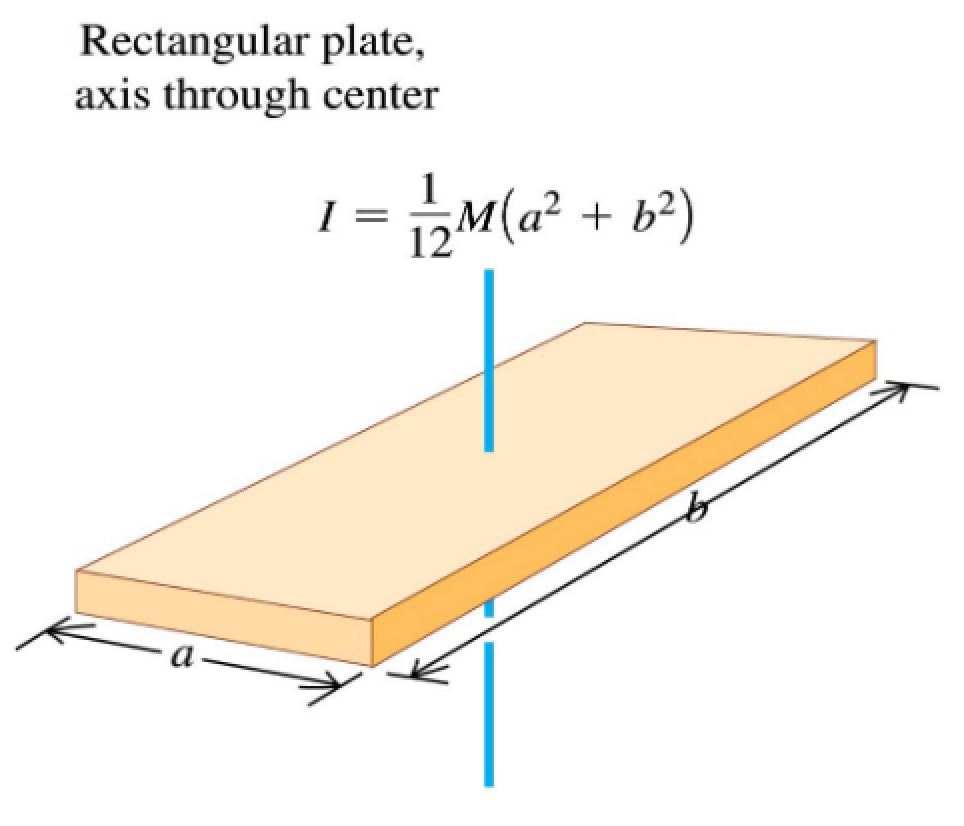
\includegraphics[width = 0.74\linewidth]{rectangular-plate-moi-1}
  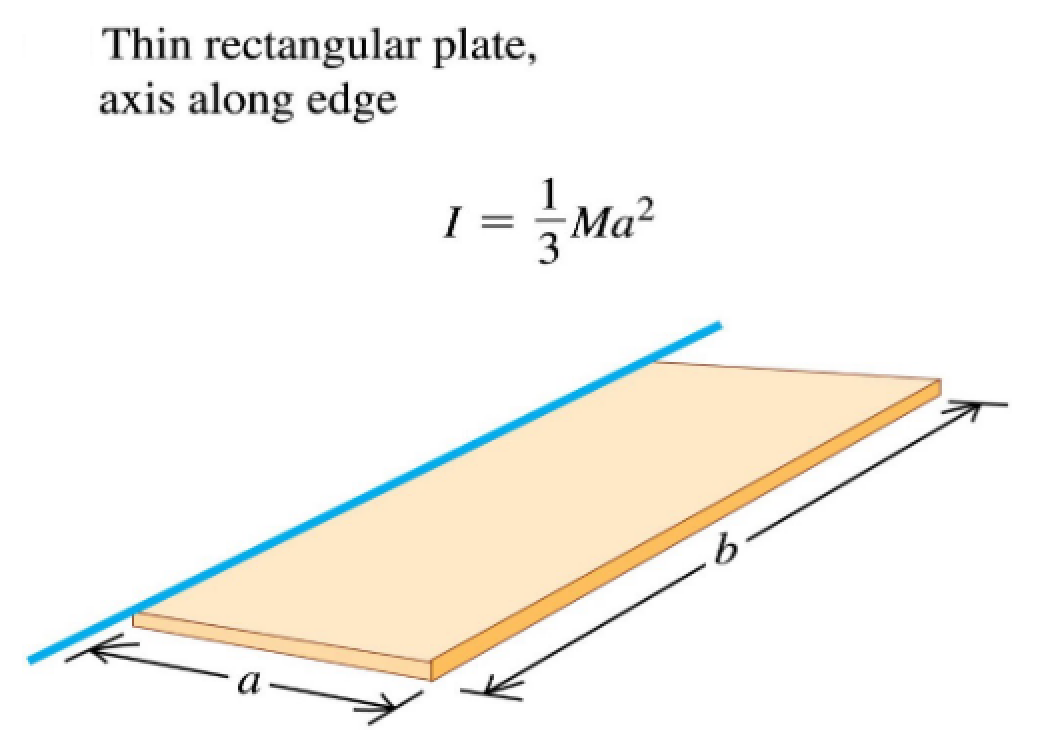
\includegraphics[width = 0.74\linewidth]{rectangular-plate-moi-2}

  % Sphere
  \begin{tabular}{c}
    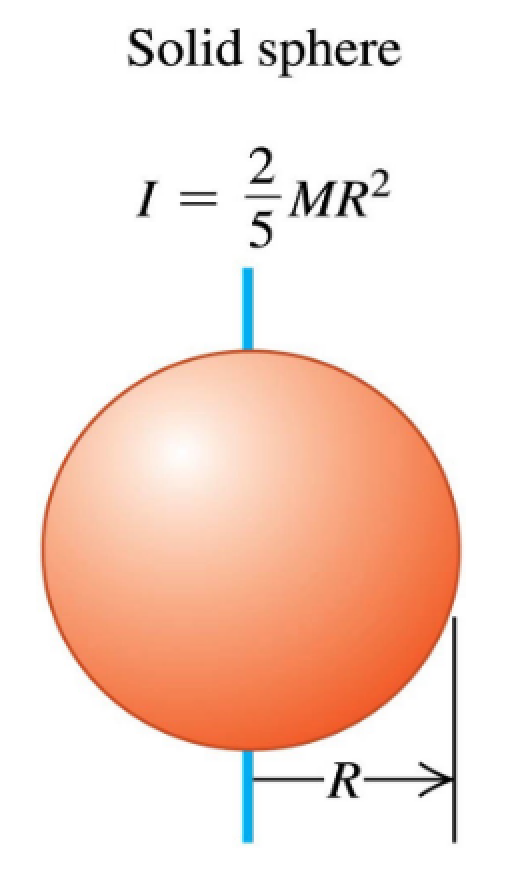
\includegraphics[width = 0.5\linewidth]{solid-sphere-moi}
    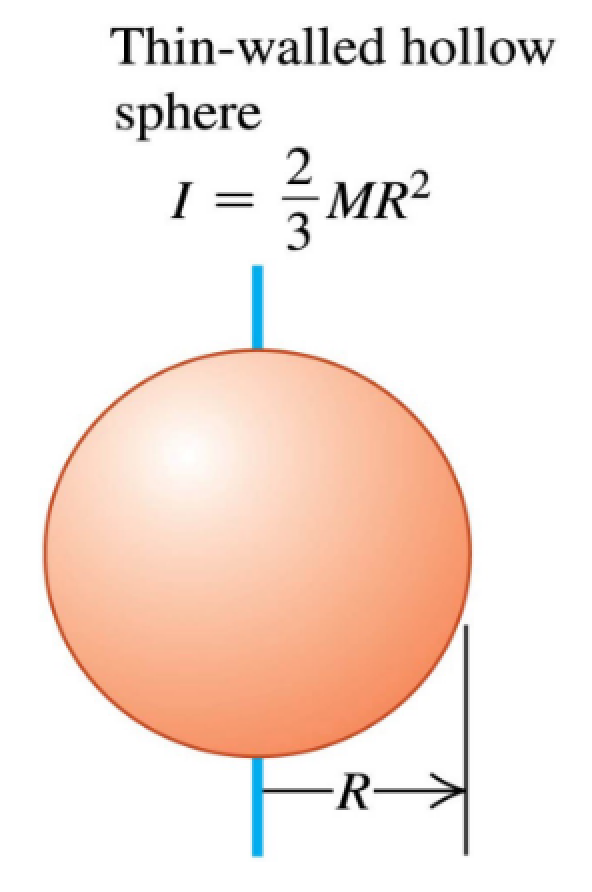
\includegraphics[width = 0.5\linewidth]{thin-walled-hollow-sphere-moi}
  \end{tabular}

  % Cylinder
  \begin{tabular}{c}
    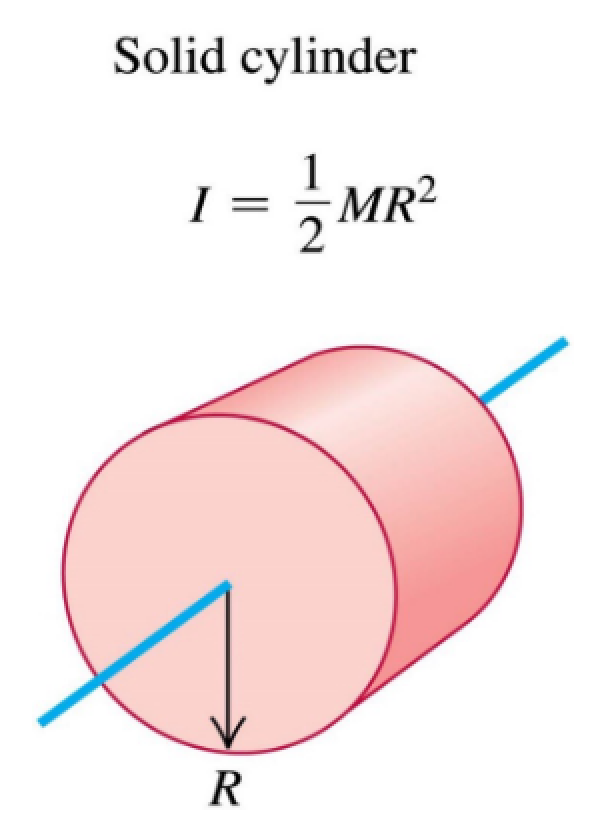
\includegraphics[width = 0.33333333333333\linewidth]{solid-cylinder-moi}
    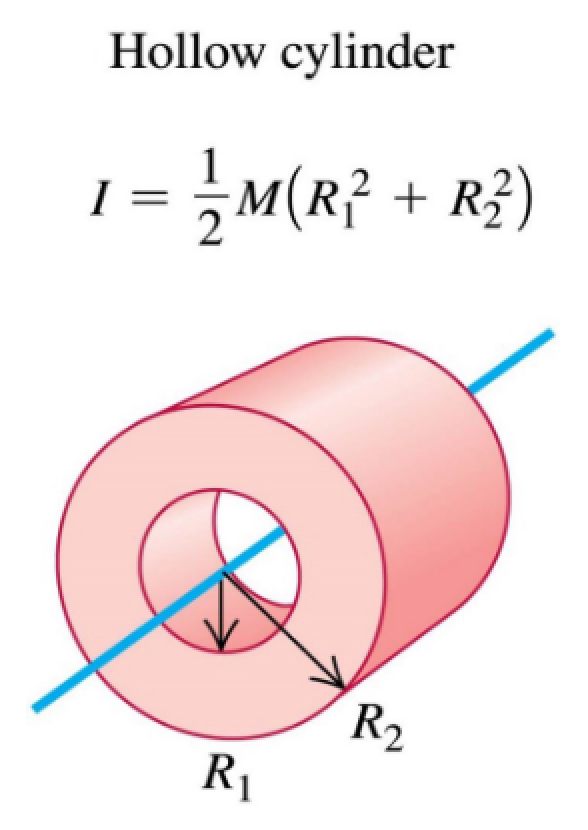
\includegraphics[width = 0.33333333333333\linewidth]{hollow-cylinder-moi}
    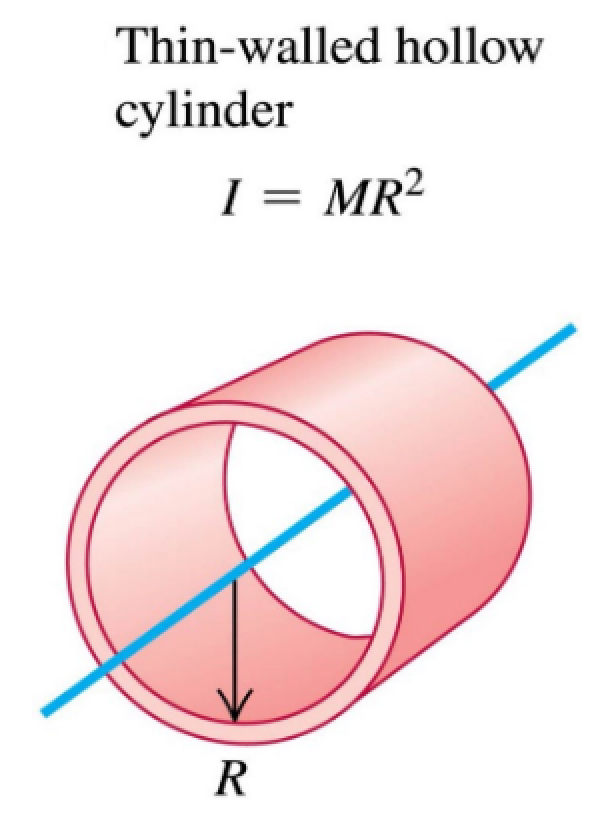
\includegraphics[width = 0.33333333333333\linewidth]{thin-walled-hollow-cylinder-moi}
  \end{tabular}

  % Slender rod
  \begin{tabular}{c}
    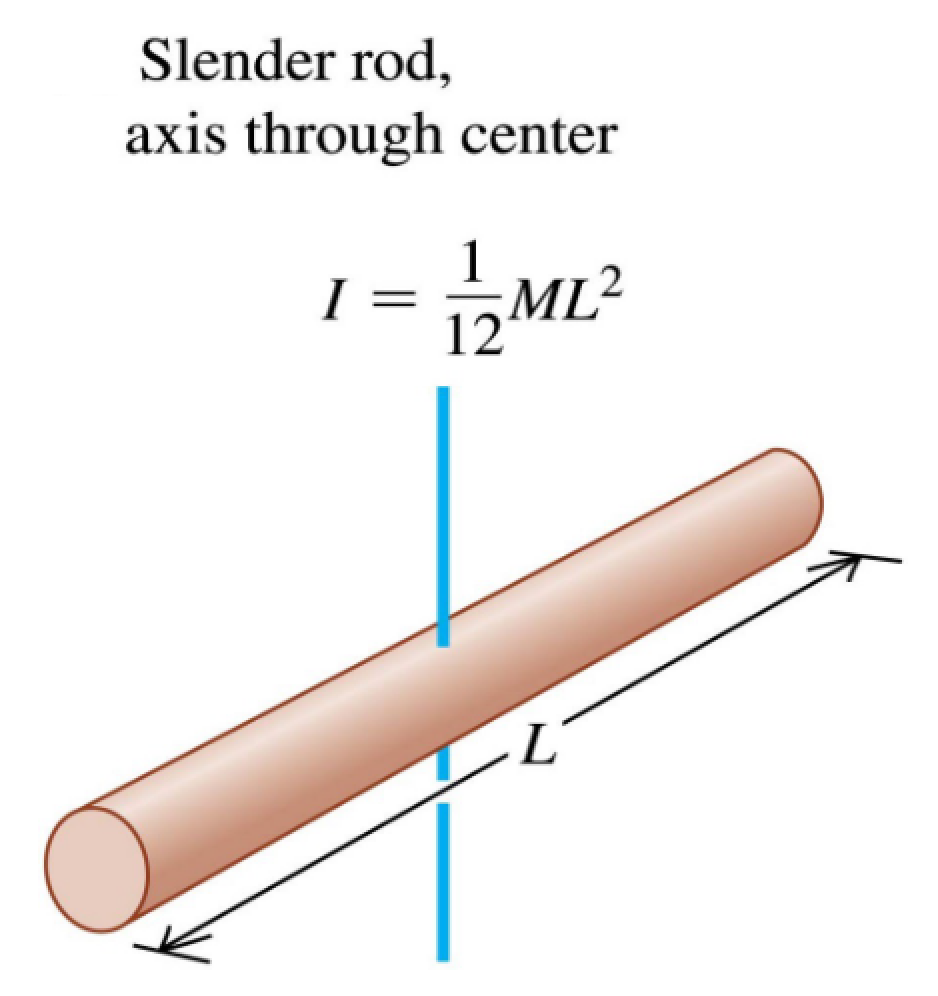
\includegraphics[width = 0.5\linewidth]{slender-rod-moi-1}
    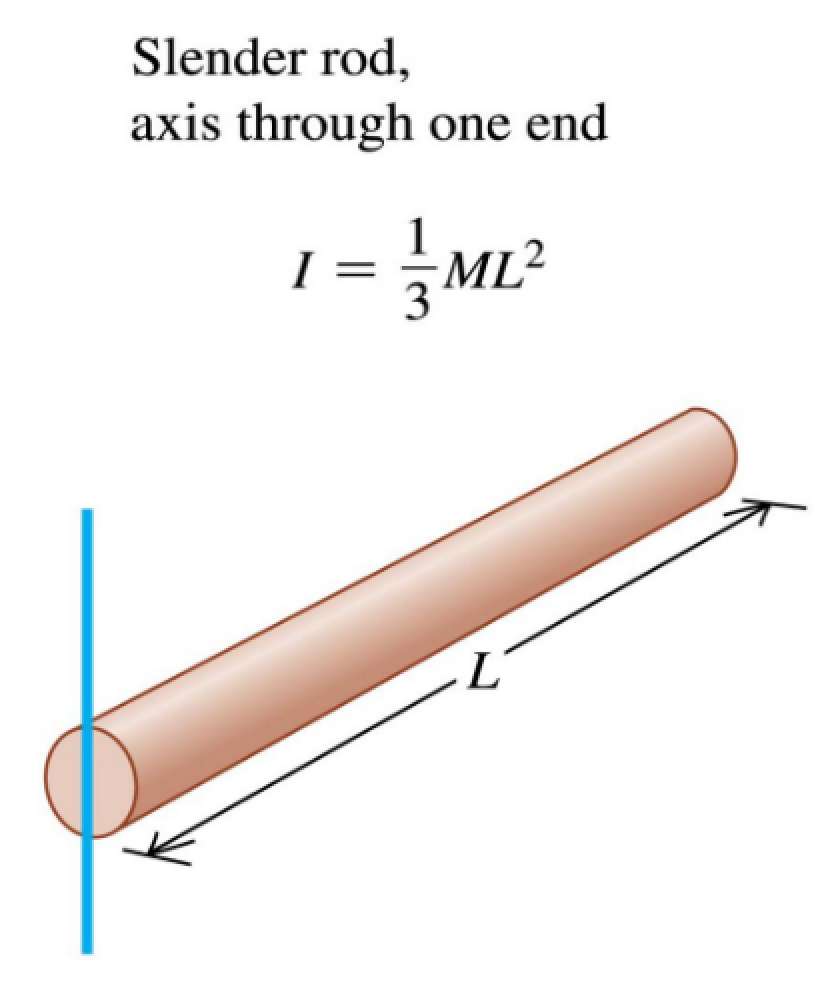
\includegraphics[width = 0.5\linewidth]{slender-rod-moi-2}
  \end{tabular}


  \section{Coordinates}
  Polar coordinates: \\
  \(x = r \cos \theta, \quad y = r \sin \theta\)

  Cylindrical coordinates: \\
  \(x = r \cos \theta, \quad y = r \sin \theta, \quad z = z\)

  Spherical coordinates: \\
  \(x = r \sin \theta \cos \phi\) \\
  \(y = r \sin \theta \sin \phi\) \\
  \(z = r \cos \theta\)


  \section{Steps}

  \subsection{Figuring out the motion of objects relative to an attached frame of reference}
  \(\lozenge\) Look at the length of the line with respect to the new origin of the attached frame of reference. \\
  \(\lozenge\) If the length of the line is constant, as in it doesn't change with time, then the motion of the object is likely a circular motion. \\
  \(\lozenge\) To confirm if the object is truly in circular motion, look at the angle the object makes with the origin of the attached frame. \\
  \(\lozenge\) This angle can be derived from the angle of the object with respect to the origin in the absolute frame. \\
  \(\lozenge\) If the angle is variable, as in it changes with time, then the object is circular motion. \\\\
  \(\lozenge\) Otherwise, if the angle is constant and doesn't change with time, then the object is not moving at all in the attached frame of reference.

  \subsection{Determining friction direction}
  \(\lozenge\) Get the relative velocity of the object with respect to the other object that it is in contact with, and hence experiencing friction due to that contact. \\
  \(\lozenge\) The friction direction will always be opposite in direction to the obtained relative velocity.

  \subsection{Steps to solve collision problems}
  \(\lozenge\) Set coordinates of the direction parallel (\(\hat{e}_n\)) and perpendicular (\(\hat{e}_t\)) to the impact, i.e. express \(\hat{i}\) and \(\hat{j}\) in terms of \(\hat{e}_n\) and \(\hat{e}_t\). \\
  \(\lozenge\) Set the restitution equation in the direction parallel to the impact (\(\hat{e}_n\) direction). \\
  \(\lozenge\) The direction perpendicular to the impact (\(\hat{e}_t\) direction) has no net force, and hence there is no change in velocities in that direction. \\
  \(\lozenge\) Gravitational force is negligible during the collision as the impact forces are relatively large. \\
  \(\lozenge\) Analyse the directions of the impact force and constrains to find the direction in which the net force of the system is zero. Apply the conservation of linear momentum in that direction.

  \subsection{Steps to solve pulley problems}
  \(\lozenge\) \textbf{Break down} the system into individual objects. \\
  \(\lozenge\) Set the kinetic equation for each object.
  \[F = ma \quad \text{and} \quad M = I \alpha \]
  \(\lozenge\) Find the relationship between the accelerations, the work done, or the energies. \\
  \(\lozenge\) Solve all the equations.

  \subsection{Steps to find centre of mass}
  \(\lozenge\) For discrete masses, treat holes as a mass but subtract them. \\
  \(\lozenge\) For continuous masses, change \(dm\) into something \(\times\) the given quantity, like \(\rho \, dV, \rho h \, dA, 2 \pi r \rho h \, dr\) for a cylinder.

  \subsection{Steps to find moment of inertia}
  \(\lozenge\) Find a symmetrical axis of rotation. \\
  \(\lozenge\) For continuous masses, change \(dm\) into something \(\times\) the given quantity, like \(\rho \, dV, \rho h \, dA, 2 \pi r \rho h \, dr\) for a cylinder. \\
  \(\lozenge\) Use parallel or perpendicular axis theorem to find the MOI about the actual axis of rotation if necessary.




  \section{Maths}

  \subsection{Derivatives}

  Chain rule: \\
  \(\frac{dz}{dx} = \frac{dz}{dy} \cdot \frac{dy}{dx}\)

  Product rule: \\
  \(\frac{d}{dx} (u \cdot v) = \frac{du}{dx} \cdot v + u \cdot \frac{dv}{dx}\)

  Quotient rule: \\
  \(\frac{d}{dx} \left(\frac{f(x)}{g(x)} \right) = \frac{f'(x) g(x) - f(x) g'(x)}{g(x)^2}\)

  Standard derivatives: \\
  \(\frac{d}{dx} \left(\sin x \right) = \cos x\) \\
  \(\frac{d}{dx} \left(\cos x \right) = - \sin x\) \\
  \(\frac{d}{dx} \left(\arcsin x \right) = \frac{1}{\sqrt{1 - x^2}}\) \\
  \(\frac{d}{dx} \left(\arccos x \right) = - \frac{1}{\sqrt{1 - x^2}}\) \\
  \(\frac{d}{dx} \left(\arctan x \right) = \frac{1}{1 + x^2}\) \\
  \(\frac{d}{dx} \left(\csc x \right) = - \csc x \cot x\) \\
  \(\frac{d}{dx} \left(\sec x \right) = \sec x \tan x\)


  \subsection{Integrals}
  \(\int \sin x \, dx = - \cos x\) \\
  \(\int \cos x \, dx = \sin x\) \\
  \(\int \frac{1}{x^2 + a^2} \, dx = \frac{1}{a} \arctan \left(\frac{x}{a} \right)\) \\
  \(\int \frac{1}{\sqrt{a^2 - x^2}} \, dx = \arcsin \left(\frac{x}{a} \right)\) \\
  \(\int \frac{1}{x^2 - a^2} \, dx = \frac{1}{2a} \ln \left|\frac{x - a}{x + a} \right|\) \\
  \(\int \frac{1}{a^2 - x^2} \, dx = \frac{1}{2a} \ln \left|\frac{a + x}{a - x} \right|\) \\
  \(\int \frac{1}{\sqrt{x^2 - a^2}} \, dx = \ln \left|\sqrt{x^2 - a^2} + x \right|\) \\
  \(\int \tan x \, dx = \ln |\sec x|\) \\
  \(\int \cot x \, dx = \ln |\sin x|\) \\
  \(\int \csc x \, dx = - \ln |\csc x + \cot x|\) \\
  \(\int \sec x \, dx = - \ln |\sec x + \tan x|\)


  \subsection{Trigonometric identities}

  Quotient identities: \\
  \(\tan \theta = \frac{\sin \theta}{\cos \theta}\) \\
  \(\cot \theta = \frac{\cos \theta}{\sin \theta}\)

  Reciprocal identities: \\
  \(\sin \theta = \frac{1}{\csc \theta}\) \\
  \(\csc \theta = \frac{1}{\sin \theta}\) \\
  \(\cos \theta = \frac{1}{\sec \theta}\) \\
  \(\sec \theta = \frac{1}{\cos \theta}\) \\
  \(\tan \theta = \frac{1}{\cot \theta}\) \\
  \(\cot \theta = \frac{1}{\tan \theta}\)

  Pythagorean identities: \\
  \(\sin^2 \theta + \cos^2 \theta = 1\) \\
  \(\sec^2 \theta - \tan^2 \theta = 1\) \\
  \(\csc^2 \theta - \cot^2 \theta = 1\)

  Even/odd identities: \\
  \(\sin(- \theta) = - \sin \theta\) \\
  \(\cos (- \theta) = \cos \theta\) \\
  \(\tan(- \theta) = - \tan \theta\) \\
  \(\cot (- \theta) = - \cot \theta\) \\
  \(\csc(- \theta) = - \csc \theta\) \\
  \(\sec (- \theta) = \sec \theta\)

  Co-function identities: \\
  \(\sin \left(\frac{\pi}{2} - \theta \right) = \cos \theta\) \\
  \(\cos \left(\frac{\pi}{2} - \theta\right) = \sin \theta \) \\
  \(\tan \left(\frac{\pi}{2} - \theta \right) = \cot \theta\) \\
  \(\cot \left(\frac{\pi}{2} - \theta\right) = \tan \theta \) \\
  \(\csc \left(\frac{\pi}{2} - \theta \right) = \sec \theta\) \\
  \(\sec \left(\frac{\pi}{2} - \theta\right) = \csc \theta \) \\
  \(\frac{\pi}{2} \text{ radians} = 90^{\circ}\)

  Sum/difference identities: \\
  \(\sin (\theta \pm \phi) = \sin \theta \cos \phi \pm \cos \theta \sin \phi\) \\
  \(\cos (\theta \pm \phi) = \cos \theta \cos \phi \mp \sin \theta \sin \phi\) \\
  \(\tan (\theta \pm \phi) = \frac{\tan \theta \pm \tan \phi}{1 \mp \tan \theta \tan \phi}\)

  Double angle identities: \\
  \(\sin (2 \theta) = 2 \sin \theta \cos \theta\) \\
  \(\cos (2 \theta) = \cos^2 \theta - \sin^2 \theta\) \\
  \(\cos (2 \theta) = 2 \cos^2 \theta - 1\) \\
  \(\cos (2 \theta) = 1 - 2 \sin^2 \theta\) \\
  \(\tan (2 \theta) = \frac{2 \tan \theta}{1 - \tan^2 \theta}\)

  Half angle identities: \\
  \(\sin^2 \theta = \frac{1 - \cos (2 \theta)}{2}\) \\
  \(\cos^2 \theta = \frac{1 + \cos (2 \theta)}{2}\) \\
  \(\tan^2 \theta = \frac{1 - \cos (2 \theta)}{1 + \cos (2 \theta)}\)

  Sum to product of 2 angles: \\
  \(\sin \theta + \sin \phi = 2 \sin \left( \frac{\theta + \phi}{2} \right) \cos \left( \frac{\theta - \phi}{2} \right)\) \\
  \(\sin \theta - \sin \phi = 2 \cos \left( \frac{\theta + \phi}{2} \right) \sin \left( \frac{\theta - \phi}{2} \right)\) \\
  \(\cos \theta + \cos \phi = 2 \cos \left( \frac{\theta + \phi}{2} \right) \cos \left( \frac{\theta - \phi}{2} \right)\) \\
  \(\cos \theta - \cos \phi = - 2 \sin \left( \frac{\theta + \phi}{2} \right) \sin \left( \frac{\theta - \phi}{2} \right)\)

  Product to sum of 2 angles: \\
  \(\sin \theta \sin \phi = \frac{\cos (\theta - \phi) - \cos (\theta + \phi)}{2}\) \\
  \(\cos \theta \cos \phi = \frac{\cos (\theta - \phi) + \cos (\theta + \phi)}{2}\) \\
  \(\sin \theta \cos \phi = \frac{\sin (\theta + \phi) + \sin (\theta - \phi)}{2}\) \\
  \(\cos \theta \sin \phi = \frac{\sin (\theta + \phi) - \sin (\theta - \phi)}{2}\)

  Law of sines: \\
  \(\frac{a}{\sin A} = \frac{b}{\sin B} = \frac{c}{\sin C}\)

  Law of cosines: \\
  \(a^2 = b^2 + c^2 - 2bc \cos A\)

  Area of a triangle: \\
  \(A = \frac{1}{2} ab \sin C\)

\end{multicols*}
\end{document}
